\documentclass[12pt,a4paper,austrian]{article}
\usepackage{graphicx}
\usepackage[austrian, english]{babel}
\usepackage[utf8]{inputenc}
%\usepackage{listings}
\usepackage{multirow}
\usepackage{epstopdf}
\usepackage{amsmath}
\usepackage{amssymb} % fuer Mengen \N, Q, C, R
\usepackage{matlab-prettifier}
\graphicspath{{./fig/}}

\usepackage[colorlinks=true, pdfborder={0 0 0}, linkcolor=red]{hyperref}
\usepackage{float}


%% Satzspiegel
\setlength{\hoffset}{-1in} \setlength{\textwidth}{18cm}
\setlength{\oddsidemargin}{1.5cm}
\setlength{\evensidemargin}{1.5cm}
\setlength{\marginparsep}{0.7em}
\setlength{\marginparwidth}{0.5cm}

\setlength{\voffset}{-1.9in}
\setlength{\headheight}{12pt}
\setlength{\topmargin}{2.6cm}
   \addtolength{\topmargin}{-\headheight}
\setlength{\headsep}{3.5cm}
   \addtolength{\headsep}{-\topmargin}
   \addtolength{\headsep}{-\headheight}
\setlength{\textheight}{27cm}

%% How should floats be treated?
\setlength{\floatsep}{12 pt plus 0 pt minus 8 pt}
\setlength{\textfloatsep}{12 pt plus 0pt minus 8 pt}
\setlength{\intextsep}{12 pt plus 0pt minus 8 pt}

\tolerance2000
\emergencystretch20pt

%% Text appearence
% English text
\newcommand{\eg}[1]%
  {\selectlanguage{english}\textit{#1}\selectlanguage{austrian}}

\newcommand{\filename}[1]
  {\begin{small}\texttt{#1}\end{small}}

\newcommand\IFT{\unitlength1mm\begin{picture}(10,2) \put (1,1)
{\circle{1.7}} \put(2,1){\line(1,0){5}} \put(8,1)
{\circle*{1.7}}\end{picture}}
\newcommand\FT{\unitlength1mm\begin{picture}(10,2) \put (1,1)
{\circle*{1.7}} \put(2,1){\line(1,0){5}} \put(8,1)
{\circle{1.7}}\end{picture}}

% A box for multiple choice problems
\newcommand{\choicebox}{\fbox{\rule{0pt}{0.5ex}\rule{0.5ex}{0pt}}}

\newenvironment{wahrfalsch}%
  {\bigskip\par\noindent\makebox[1cm][c]{richtig}\hspace{3mm}\makebox[1cm][c]{falsch}
   \begin{list}%
   {\makebox[1cm][c]{\choicebox}\hspace{3mm}\makebox[1cm][c]{\choicebox}}%
   {\setlength{\labelwidth}{2.31 cm}\setlength{\labelsep}{3mm}
    \setlength{\leftmargin}{2.61 cm}\setlength{\listparindent}{0pt}
    \setlength{\itemindent}{0pt}}%
  }
  {\end{list}}

\newcounter{theaufgabe}\setcounter{theaufgabe}{1}
\newenvironment{aufgabe}[1]%
  {\bigskip\par\noindent\begin{nopagebreak}
   \textsf{\textbf{Exercise \arabic{theaufgabe}}}\quad
      \textsf{\textit{#1}}\\*[1ex]%
\stepcounter{theaufgabe}\hspace{2ex}\end{nopagebreak}}
  {\par\pagebreak[2]}

% Innerhalb der Aufgaben erfolgt die weitere Unterteilung mittels einer
% enumerate Umgebung, die allerdings a), b),... zaehlen soll.
\renewcommand{\labelenumi}{\alph{enumi})}
\renewcommand{\labelenumii}{\arabic{enumii})}

% A box to tick for everything which has to done
\newcommand{\abgabe}{\marginpar{$\Box$}}
% Margin paragraphs on the left side
\reversemarginpar

% Language for listings
%\lstset{language=Vhdl,
%  basicstyle=\small\tt,
 % keywordstyle=\tt\bf,
 % commentstyle=\sl}

% No indention
\setlength{\parindent}{0.0cm}
% Don't number sections
\setcounter{secnumdepth}{0}

% prints a predefined preamble
% done this so that we don't have all the code later in the file
\newcommand{\printpreamble}{
  \pagestyle{plain}
  \thispagestyle{empty}
  \noindent
  \begin{minipage}[b][4cm]{1.0\textwidth}  
  \begin{center}
  \begin{bf} 
  \begin{large} Digital Signal Processing SS 2024 -- Exercise~5\end{large} \\
  \vspace{0.3cm}
  \begin{Large} Digital Signal Processing Tutorial  \end{Large} \\
  \vspace{0.3cm}
  \end{bf}
  \begin{large} 
  Group 23\\
  Aaron Zettler, 12105021\\
  Pascal Pilz, 12111234\\
  \end{large} 
  \end{center}
  \end{minipage}
  
  \noindent \rule[0.8em]{\textwidth}{0.12mm}\\[-0.5em]
}

%% Beginning of the text
%=======================================================================================

\begin{document}
\printpreamble

\begin{aufgabe}{} % Exercise 3 ---------------------------------------------------------

\end{aufgabe} \pagebreak

\begin{aufgabe}{} % Exercise 2 ---------------------------------------------------------

  We are given the difference equation 
  $$
  y[n] = x[n] - \frac{1}{15} y[n-1] + \frac25 y[n-2].
  $$

  \begin{enumerate}
    \item We sketch the corresponding block diagram:
  
    \begin{center}
      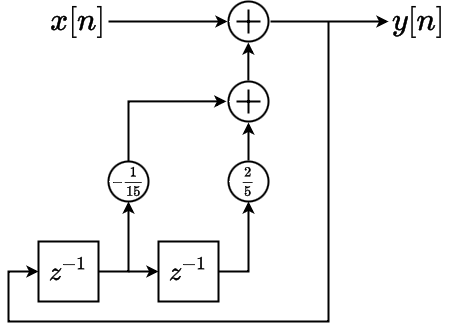
\includegraphics[width=0.4\textwidth]{../Ex02_a.png}
    \end{center}

    \item The system is an IIR Filter. This is because in the difference equation we have non-zero $a$ coefficients, i.e., it is a recursive filter.

    \item To find the transfer function, we first need to transform the system to the $z$-domain. For the transformation we use the linearity of the $z$-transformation. We assume that the signal is causal, i.e., $x[n] = y[n] = 0$ for $n < 0$.
    \begin{align}
      & y[n]
      = x[n] - \frac{1}{15} y[n-1] + \frac25 y[n-2] \\
      &\hspace*{0.6em}\rotatebox{90}{\FT} \\
      & Y(z)
      = X(z) - \frac{1}{15} z^{-1} Y(z) + \frac25 z^{z-2} Y(z)
      \quad \Longleftrightarrow \\
      & Y(z) \left( 1 + \frac{1}{15} z^{-1} - \frac25 z^{-2} \right)
      = X(z)
      \quad \Longleftrightarrow \\
      & Y(z)
      = \left( 1 + \frac{1}{15} z^{-1} - \frac25 z^{-2} \right)^{-1} X(z)
    \end{align}

    We can see that the transfer function $H(z) = \frac{Y(z)}{X(z)}$ is given by

    \begin{align}
      H(z)
      & = \left( 1 + \frac{1}{15} z^{-1} - \frac25 z^{-2} \right)^{-1} \\
      & = \frac{1}{1 + \frac{1}{15} z^{-1} - \frac25 z^{-2}} \\
      & = \frac{1}{1 + \frac{1}{15} z^{-1} - \frac25 z^{-2}} \frac{z^2}{z^2} \\
      & = \frac{z^2}{z^2 + \frac{1}{15} z - \frac25} \\
    \end{align}

    \item The roots of the numerator are clearly 0. The roots of the denominator can be determined from $z^2 + \frac{1}{15} z - \frac25 = 0$:
    \begin{align}
       z_{1,2} 
       & = - \frac{1}{30} \pm \sqrt{\frac{1}{1125} - \frac{8}{20}} \\
       & = - \frac{1}{30} \pm j \sqrt{\frac{8980}{22500}} \\
       & = - \frac{1}{30} \pm j \frac{\sqrt{8980}}{150} \\
       & \approx - 0.0333 \pm j 0.0574
    \end{align}

    You can see a sketch of the pole-zero map:
    \begin{center}
      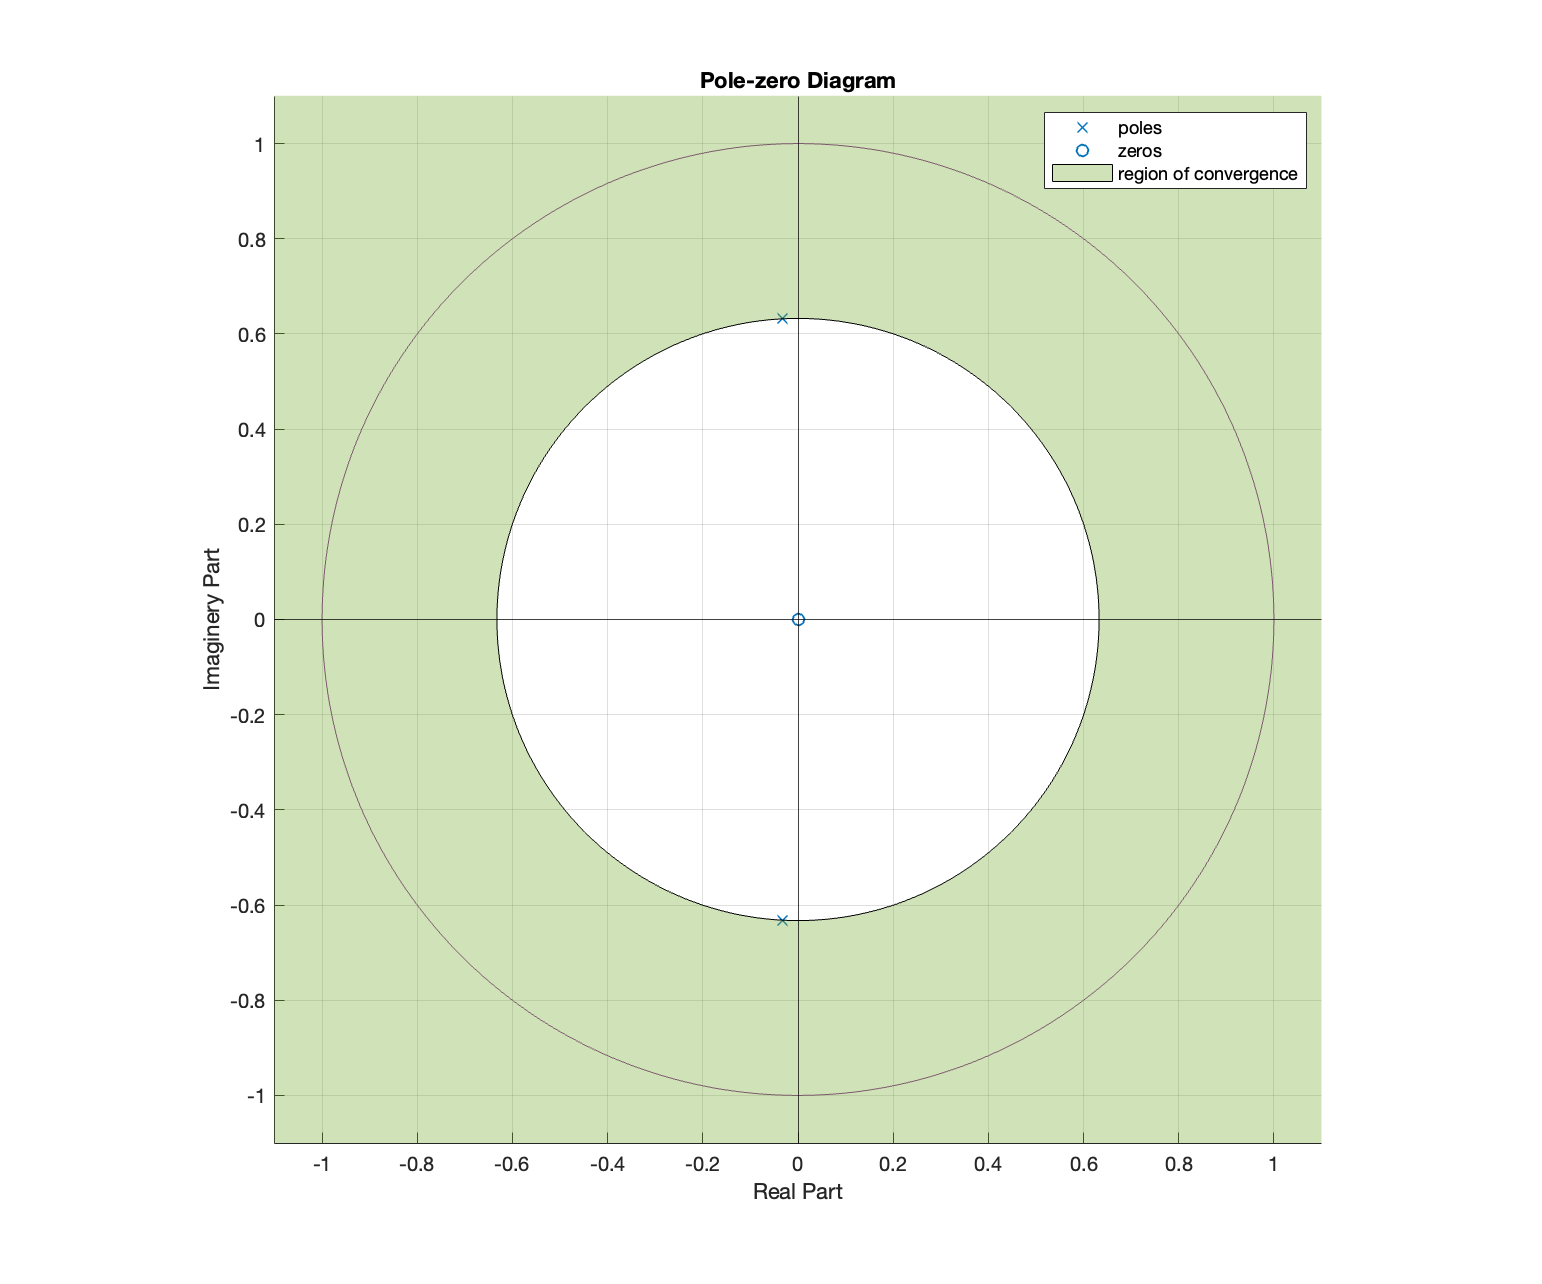
\includegraphics[width=0.8\textwidth]{../Ex02_d.png}
    \end{center}

    \item The system is stable. This can be seen by the region of convergence including the unit circle.

  \end{enumerate}

\end{aufgabe} \pagebreak


\begin{aufgabe}{} % Exercise 3 ---------------------------------------------------------

  We are given a set of poles and zeros:
  \begin{itemize}
    \item Zeros: $N_1 = -1$, $N_2 = j$, $N_3 = -j$
    \item Poles: $P_1 = 0$, $P_2 = 0.75 + j0.25$, $P_3 = 0.27 - 0.25j$
  \end{itemize}

  \begin{enumerate}
    \item This filter has only real coefficients, since when we express the transfer function in the pole-zero representation then we can see that the numerator and denominator both contain a complex number and their corresponding conjugate, meaning that when we multiply it out we will be left with only real coefficients.

    \item You can see a sketch of the pole-zero map:
    \begin{center}
      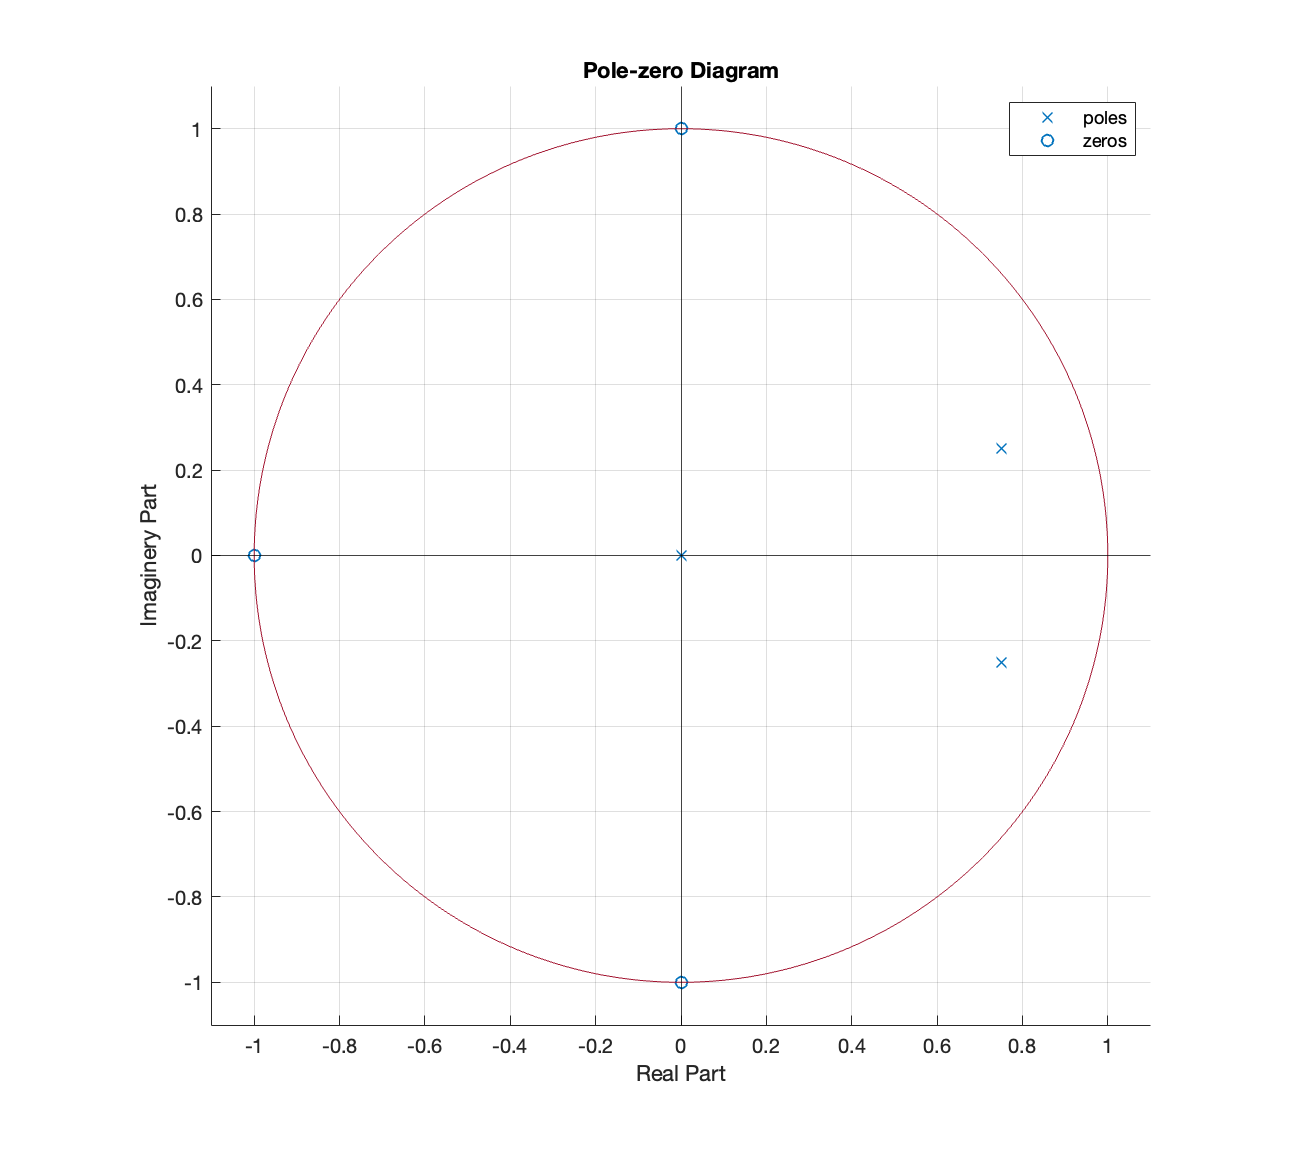
\includegraphics[width=0.8\textwidth]{../Ex03_b.png}
    \end{center}

    \item The transfer function can be obtained by writing it first in pole-zero representation and then multiplying out the clauses :
    \begin{align}
      H(z)
      &= b_0 z^{M-N} \frac{(z-N_1)(z-N_2)(z-N_3)}{(z-P_1)(z-P_2)(z-P_3)} \\
      &= b_0 \frac{(z+1)(z+j)(z-j)}{z(0.75+j0.25)(0.27-0.25j)} \\
      &= b_0 \frac{z^3 + z^2 + z + 1}{z^3 - 1.5z^2 + 0.625z} \\
      &= \frac{b_0z^3 + b_0z^2 + b_0z + b_0}{z^3 - 1.5z^2 + 0.625z} \\
      &= \frac{b_0 + b_0z^{-1} + b_0z^{-2} + b_0z^{-3}}{1 - 1.5z^{-1} + 0.625z^{-2}} \\
    \end{align}

    \item The block diagram of a direct-form-I implementation of the filter can be seen:
    \begin{center}
      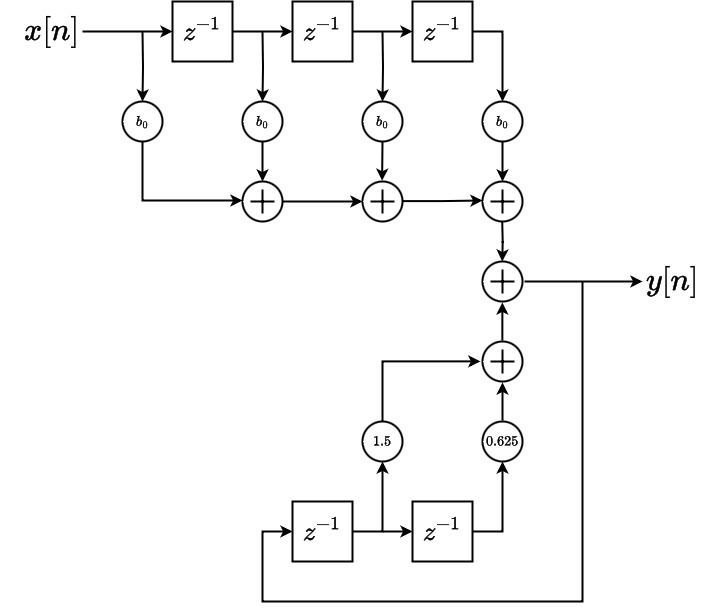
\includegraphics[width=0.6\textwidth]{../Ex03_d.png}
    \end{center}

    \item The magnitude and phase response can be seen:
    
    \begin{center}
      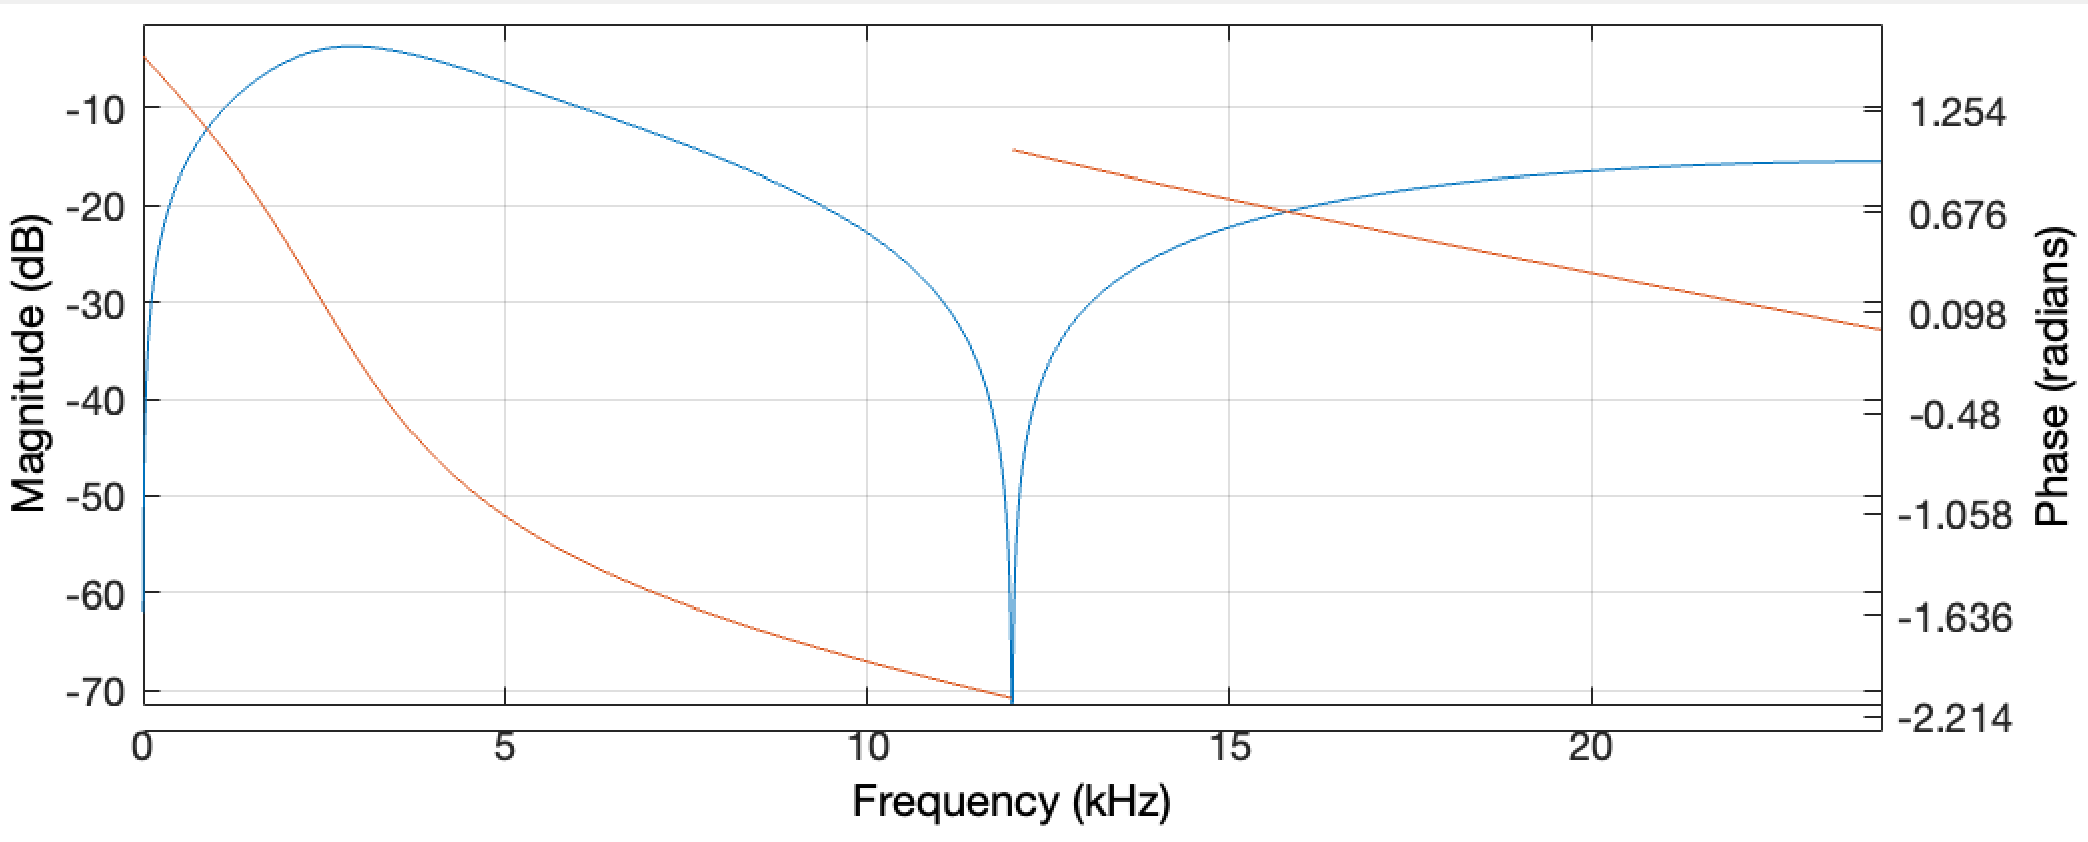
\includegraphics[width=0.8\textwidth]{../Ex03_e.png}
    \end{center}

    \item The impulse response for $0 \leq n \leq 50$ can be seen:

    \begin{center}
      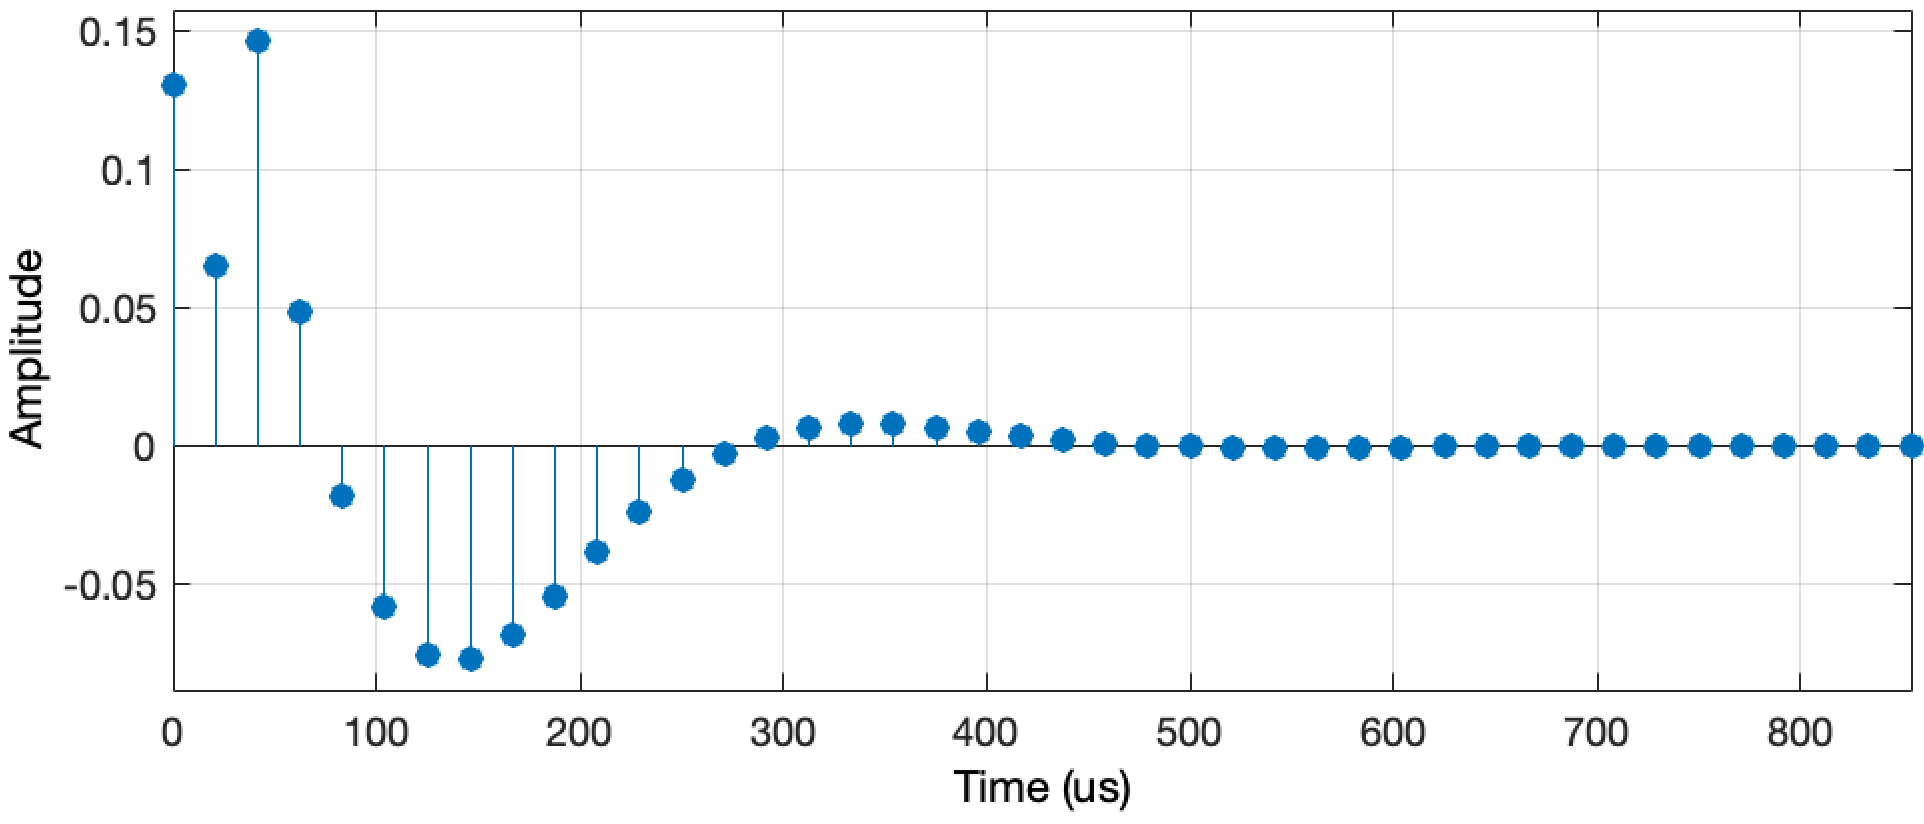
\includegraphics[width=0.8\textwidth]{../Ex03_f.png}
    \end{center}

  \end{enumerate}

\end{aufgabe} \pagebreak


\begin{aufgabe}{} % Exercise 4 ---------------------------------------------------------

\end{aufgabe} \pagebreak


\end{document}
